\documentclass[11pt, a4paper]{article}

% --- Packages ---
\usepackage[margin=2.5cm]{geometry}
\usepackage[T1]{fontenc}
\usepackage[utf8]{inputenc}
\usepackage{lmodern}
\usepackage{microtype}
\usepackage{amsmath, amssymb, amsthm}
\usepackage{mathtools}
\usepackage{booktabs}
\usepackage{array}
\usepackage{tabularx}
\usepackage{xcolor}
\usepackage{tikz}
\usetikzlibrary{arrows.meta, positioning, shapes.geometric, calc, fit, backgrounds}
\usepackage{hyperref}
\usepackage{enumitem}
\usepackage{fancyhdr}
\usepackage{titlesec}
\usepackage{mdframed}
\usepackage{parskip}
\usepackage{algorithm}
\usepackage{algpseudocode}

% --- Colors ---
\definecolor{accentblue}{RGB}{30, 100, 180}
\definecolor{accentgray}{RGB}{90, 90, 90}
\definecolor{alertbg}{RGB}{255, 248, 230}
\definecolor{alertborder}{RGB}{220, 160, 30}
\definecolor{greenbg}{RGB}{235, 248, 235}
\definecolor{greenborder}{RGB}{60, 160, 60}
\definecolor{src_col}{RGB}{180, 60, 60}
\definecolor{sink_col}{RGB}{30, 90, 180}
\definecolor{int_col}{RGB}{40, 140, 60}
\definecolor{comp_col}{RGB}{150, 80, 180}
\definecolor{bordercolor}{RGB}{200,200,200}
\definecolor{codebg}{RGB}{248,248,248}

% --- Theorem environments ---
\theoremstyle{plain}
\newtheorem{theorem}{Theorem}[section]
\newtheorem{lemma}[theorem]{Lemma}
\newtheorem{corollary}[theorem]{Corollary}
\theoremstyle{definition}
\newtheorem{definition}[theorem]{Definition}
\newtheorem{example}[theorem]{Example}
\theoremstyle{remark}
\newtheorem{remark}[theorem]{Remark}
\newtheorem{proposition}[theorem]{Proposition}

% --- mdframed boxes ---
\newmdenv[backgroundcolor=alertbg, linecolor=alertborder, linewidth=1.5pt,
  innerleftmargin=10pt, innerrightmargin=10pt,
  innertopmargin=8pt,  innerbottommargin=8pt,
  skipabove=8pt, skipbelow=8pt]{notebox}

\newmdenv[backgroundcolor=greenbg, linecolor=greenborder, linewidth=1.5pt,
  innerleftmargin=10pt, innerrightmargin=10pt,
  innertopmargin=8pt,  innerbottommargin=8pt,
  skipabove=8pt, skipbelow=8pt]{keybox}

% --- Headers ---
\pagestyle{fancy}
\fancyhf{}
\fancyhead[L]{\small\textcolor{accentgray}{Transistor Switching Network Synthesis}}
\fancyhead[R]{\small\textcolor{accentgray}{\leftmark}}
\fancyfoot[C]{\small\thepage}
\renewcommand{\headrulewidth}{0.4pt}

% --- Section styling ---
\titleformat{\section}
  {\large\bfseries\color{accentblue}}{\thesection.}{0.6em}{}
  [\vspace{-2pt}\rule{\linewidth}{0.8pt}\vspace{4pt}]
\titleformat{\subsection}
  {\normalsize\bfseries\color{accentblue!80!black}}{\thesubsection}{0.6em}{}
\titleformat{\subsubsection}
  {\normalsize\bfseries\color{accentgray}}{\thesubsubsection}{0.6em}{}

% --- Hyperref ---
\hypersetup{colorlinks=true, linkcolor=accentblue, urlcolor=accentblue,
  pdftitle={Transistor Switching Network: Modeling}}

% --- Macros ---
\newcommand{\SOURCE}{\texttt{S}}
\newcommand{\SINK}{\texttt{T}}
\newcommand{\Pplus}{P^{+}}
\newcommand{\Pminus}{P^{-}}
% Time-indexed graph sets: \VG[t] -> V_{G,t},  \VG[] -> V_G
\newcommand{\VG}[1][]{V_{G\if\relax\detokenize{#1}\relax\else,#1\fi}}
\newcommand{\EG}[1][]{E_{G\if\relax\detokenize{#1}\relax\else,#1\fi}}
\newcommand{\VC}[1][]{V_{C\if\relax\detokenize{#1}\relax\else,#1\fi}}
\newcommand{\EC}[1][]{E_{C\if\relax\detokenize{#1}\relax\else,#1\fi}}
\newcommand{\GC}[1][]{\mathit{GC}\if\relax\detokenize{#1}\relax\else_{#1}\fi}
\newcommand{\nnew}{n_{\mathrm{new}}}

% ================================================================
\begin{document}

% --- Title ---
\begin{titlepage}
  \centering
  \vspace*{4cm}
  {\Huge\bfseries\color{accentblue}
    Transistor Switching Network Synthesis}\\[0.8em]
  {\Large\color{accentgray}
    Modeling, State Representation, and Generation Process}\\[2.5em]
  \rule{0.5\linewidth}{0.8pt}\\[2em]
  {\normalsize
    A formal introduction to switching networks,\\
    Boolean function representation, and the sequential\\
    generation MDP with SOP-based state initialization.\\[1em]
    \textit{TransNetGame Project}
  }
  \vfill
\end{titlepage}

\tableofcontents
\newpage

% ================================================================
\section{Switching Networks}

\subsection{Basic Definitions}

We work with $N$ Boolean input variables $\mathbf{x} = (x_1, \ldots, x_N)$.
An input pattern $\pi \in \{0,1\}^N$ assigns a concrete value to each
variable.  The \textbf{literal alphabet} is
\[
  \mathcal{L} = \{x_1,\, \lnot x_1,\, x_2,\, \lnot x_2,\,
                  \ldots,\, x_N,\, \lnot x_N\},
  \qquad |\mathcal{L}| = 2N.
\]
Literal $x_j$ evaluates to $\pi_j$ under $\pi$; literal $\lnot x_j$
evaluates to $1 - \pi_j$.

\begin{definition}[Switching Network]
A \textbf{switching network} over variables $\mathbf{x}$ is an
undirected multigraph
\[
  G = (V,\, E), \qquad
  V \supseteq \{\SOURCE,\, \SINK\}, \qquad
  E \subseteq \binom{V}{2} \times \mathcal{L},
\]
where $\SOURCE$ (source) and $\SINK$ (drain/sink) are two
distinguished terminal nodes. Every edge $(u, v, \ell) \in E$
represents a \textbf{transistor} with control literal $\ell \in
\mathcal{L}$.
\end{definition}

\begin{definition}[Conduction]
Under input pattern $\pi$, transistor $(u, v, \ell)$
\textbf{conducts} if and only if $\ell(\pi) = 1$.  Network $G$
\textbf{conducts} $\SOURCE \to \SINK$ under $\pi$ if and only if
there exists a path from $\SOURCE$ to $\SINK$ in the subgraph of
$G$ restricted to conducting transistors.
\end{definition}

\subsection{Correctness and Safety}

Given a Boolean function $f : \{0,1\}^N \to \{0,1\}$, partition all
$2^N$ input patterns into:
\[
  \Pplus = \{\pi : f(\pi) = 1\}
  \quad(\textit{on-patterns}),
  \qquad
  \Pminus = \{\pi : f(\pi) = 0\}
  \quad(\textit{off-patterns}).
\]

\begin{definition}[Correct Implementation]
Network $G$ \textbf{correctly implements} $f$ if and only if:
\begin{align}
  \forall\,\pi \in \Pplus &:\quad
    \SOURCE \to \SINK \text{ conducts in } G \text{ under } \pi,
    \tag{Correctness} \\
  \forall\,\pi \in \Pminus &:\quad
    \SOURCE \not\to \SINK \text{ in } G \text{ under } \pi.
    \tag{Safety}
\end{align}
\end{definition}

The synthesis goal is to find a correct implementation with the
minimum number of transistors:
\[
  \min\bigl\{|E| : G = (V, E) \text{ correctly implements } f\bigr\}.
\]

\subsection{Monotonicity — A Key Structural Property}

\begin{theorem}[Monotonicity of Conducting Paths]
\label{thm:mono}
For any network $G$ and any transistor $e \notin E$,
\[
  \mathrm{Paths}(G \cup \{e\}) \supseteq \mathrm{Paths}(G),
\]
where $\mathrm{Paths}(H)$ denotes the set of $(\SOURCE,\SINK)$
conducting paths of $H$ under all patterns.
\end{theorem}

\begin{proof}
Adding a transistor can activate new paths but cannot deactivate
any existing conducting transistor.  Hence every path that existed
in $G$ still exists in $G \cup \{e\}$.
\end{proof}

\begin{corollary}[Inheritable Safety]
\label{cor:safety}
If $G$ is safe (no $\SOURCE \to \SINK$ path under any $\pi \in \Pminus$),
then $G \cup \{(u, v, \ell)\}$ is safe if and only if
$(u, v, \ell)$ does not create any $\SOURCE \to \SINK$ path under any
$\pi \in \Pminus$.
\end{corollary}

Corollary~\ref{cor:safety} means safety is an
\emph{incrementally checkable invariant}: we need only verify the
new transistor, not the entire network.

% ================================================================
\section{SOP Representation and the Series-Parallel Network}

\subsection{Sum-of-Products (SOP)}

Any Boolean function $f$ can be expressed as a disjunction of
\textbf{minterms}.  For $N$ variables, each on-pattern
$\pi = (b_1, \ldots, b_N) \in \Pplus$ uniquely corresponds to the
product term
\[
  T_\pi
  = \ell_1^\pi \cdot \ell_2^\pi \cdots \ell_N^\pi,
  \qquad
  \ell_j^\pi =
  \begin{cases}
    x_j     & \text{if } b_j = 1,\\
    \lnot x_j & \text{if } b_j = 0.
  \end{cases}
\]
The full SOP is $f = \bigvee_{\pi \in \Pplus} T_\pi$.

\subsection{Series Chain per Minterm}

Product term $T_\pi$ maps directly to a \textbf{series chain} of $N$
transistors.  Introduce $N-1$ fresh internal nodes
$c_{\pi,1}, \ldots, c_{\pi,N-1}$ and connect:
\[
  \SOURCE
    \xrightarrow{\;\ell_1^\pi\;}
  c_{\pi,1}
    \xrightarrow{\;\ell_2^\pi\;}
  c_{\pi,2}
    \;\cdots\;
  c_{\pi,N-1}
    \xrightarrow{\;\ell_N^\pi\;}
  \SINK.
\]
This chain conducts under pattern $\pi'$ if and only if every literal
$\ell_j^\pi$ evaluates to 1 under $\pi'$, which happens precisely
when $\pi' = \pi$.

\subsection{Parallel Combination: the SOP Series-Parallel Network}

\begin{definition}[SOP Network]
The \textbf{SOP series-parallel network} for $f$ is the union of
all minterm chains sharing terminal nodes $\SOURCE$ and $\SINK$:
\[
  G_{\mathrm{SOP}}(f)
  = \Bigl(
      \{\SOURCE, \SINK\}
        \cup \{c_{\pi,j} : \pi \in \Pplus,\; j = 1,\ldots,N-1\},
      \;\bigcup_{\pi \in \Pplus} \mathrm{chain}(\pi)
    \Bigr).
\]
\end{definition}

\begin{theorem}[Correctness and Safety of $G_{\mathrm{SOP}}$]
\label{thm:sop}
$G_{\mathrm{SOP}}(f)$ correctly implements $f$.
\end{theorem}

\begin{proof}
\textbf{Correctness.}
For $\pi \in \Pplus$, every literal $\ell_j^\pi$ evaluates to 1
under $\pi$, so the chain for $\pi$ is fully conducting:
$\SOURCE \to \SINK$.

\textbf{Safety.}
For $\pi' \in \Pminus$, consider any chain indexed by $\pi \in \Pplus$.
Since $\pi' \neq \pi$, they differ in at least one bit position $j^*$.
Then $\ell_{j^*}^\pi(\pi') = 0$: the $j^*$-th transistor of the
$\pi$-chain is off.  Every chain contains at least one non-conducting
transistor under $\pi'$, so no $\SOURCE \to \SINK$ path exists.
\end{proof}

The SOP network is always \emph{correct and safe by construction},
but is generally \emph{not minimal}.

\medskip
\begin{center}
\begin{tabular}{lc}
\toprule
\textbf{Quantity} & \textbf{Value} \\
\midrule
Transistors $|E_{\mathrm{SOP}}|$ & $|\Pplus| \times N$ \\
Internal nodes & $|\Pplus| \times (N-1)$ \\
\bottomrule
\end{tabular}
\end{center}

\subsection{Illustrated Example: XOR ($N=2$)}

$f(x_1,x_2) = x_1 \oplus x_2$,\;
$\Pplus = \{(1,0),\,(0,1)\}$,\;
$\Pminus = \{(0,0),\,(1,1)\}$.

$G_{\mathrm{SOP}}$ consists of two series chains in parallel:

\begin{center}
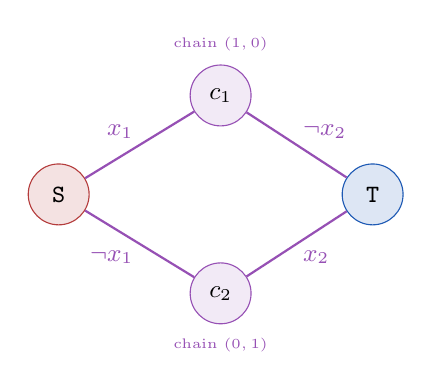
\begin{tikzpicture}[
    node distance=1.8cm and 2.4cm,
    every node/.style={font=\small},
    ns/.style={circle, draw, minimum size=22pt, inner sep=2pt},
    src/.style={ns, fill=src_col!15, draw=src_col},
    snk/.style={ns, fill=sink_col!15, draw=sink_col},
    cmp/.style={ns, fill=comp_col!12, draw=comp_col},
]
  \node[src] (S) {$\SOURCE$};
  \node[cmp, above right=0.7cm and 1.5cm of S] (c1) {$c_1$};
  \node[cmp, below right=0.7cm and 1.5cm of S] (c2) {$c_2$};
  \node[snk, right=3.2cm of S] (T) {$\SINK$};

  \draw[thick, comp_col] (S)  -- node[above left=-2pt]  {\small$x_1$}      (c1);
  \draw[thick, comp_col] (c1) -- node[above right=-2pt] {\small$\lnot x_2$}(T);
  \draw[thick, comp_col] (S)  -- node[below left=-2pt]  {\small$\lnot x_1$}(c2);
  \draw[thick, comp_col] (c2) -- node[below right=-2pt] {\small$x_2$}      (T);

  \node[above=0.05cm of c1, font=\tiny, text=comp_col] {chain $(1,0)$};
  \node[below=0.05cm of c2, font=\tiny, text=comp_col] {chain $(0,1)$};
\end{tikzpicture}
\end{center}

$|E_{\mathrm{SOP}}| = 4$ transistors,\; $|\Pplus| \times N = 2 \times 2 = 4$.
(Already optimal for XOR with $N=2$.)

% ================================================================
\section{Sequential Generation as a Markov Decision Process}

We model transistor network synthesis as a sequential decision process.
At each step the agent places one transistor; the episode terminates
when the synthesized network already covers all on-patterns.

\subsection{Two-Component State}

The state at every time step $t$ consists of two disjoint subnetworks
that together form the \textbf{unified graph} $\GC[t]$:

\begin{center}
\renewcommand{\arraystretch}{1.35}
\begin{tabularx}{\linewidth}{%
  >{\raggedright\arraybackslash}p{3.2cm}%
  >{\raggedright\arraybackslash}X%
  >{\raggedright\arraybackslash}p{4.0cm}}
\toprule
\textbf{Component} & \textbf{Definition} & \textbf{Role} \\
\midrule
Synthesized network $G_t$ &
  $(\VG[t],\,\EG[t])$;\; $\VG[0]=\{\SOURCE,\SINK\}$, $\EG[0]=\emptyset$ &
  Transistors placed by the agent so far \\[4pt]
Compensate network $C_t$ &
  $G_{\mathrm{SOP}}(f)$;\; \textit{fixed for all} $t$ &
  Full SOP network for $f$; encodes all on-patterns \\[4pt]
Unified graph $\GC[t]$ &
  $G_t \cup C_t = (\VG[t]\cup\VC[],\;\EG[t]\cup\EC[])$ &
  Full observation available to the policy \\
\bottomrule
\end{tabularx}
\end{center}

$\SOURCE$ and $\SINK$ are shared between both components.
Internal nodes of $G_t$ and $C_t$ are disjoint sets.

\subsection{The Compensate Network: Always the Full SOP}

At every step $t$, the compensate network is the \emph{complete, fixed}
SOP series-parallel network for the entire Boolean function $f$:

\begin{definition}[Compensate Network]
The compensate network is the full SOP series-parallel network for $f$
and is \emph{fixed throughout the entire episode}:
\[
  C_t = G_{\mathrm{SOP}}(\Pplus) = G_{\mathrm{SOP}}(f)
  \qquad \text{for all } t \geq 0.
\]
It contains one series chain per on-pattern in $\Pplus$, and all
chains share the terminals $\SOURCE$ and $\SINK$.
\end{definition}

\begin{keybox}
\textbf{Why always the full SOP?}

The compensate network is a \emph{fixed reference} that encodes the
complete specification of the Boolean function throughout the episode.

\begin{itemize}[leftmargin=1.5em, topsep=2pt, itemsep=0pt]
  \item \textbf{Information completeness:} $C_t$ always encodes
    \emph{every} on-pattern as an explicit series chain; the policy
    always has full knowledge of the function to be synthesized.
  \item \textbf{Structural stability:} The same series-parallel
    topology is present at every step, giving the policy a consistent
    graph structure regardless of how many transistors have been placed.
  \item \textbf{No Boolean minimization:} Building $G_{\mathrm{SOP}}(f)$
    requires only enumerating $\Pplus$; no external logic solver is needed.
\end{itemize}
\end{keybox}

The compensate network $C_t = G_{\mathrm{SOP}}(f)$ remains unchanged
from step~0 to termination.  Coverage progress is tracked separately
via $\Pplus_t \subseteq \Pplus$ (on-patterns not yet routed in $G_t$).
The episode ends when $\Pplus_t = \emptyset$, i.e.\ $G_t$ alone covers
all on-patterns.

\begin{center}
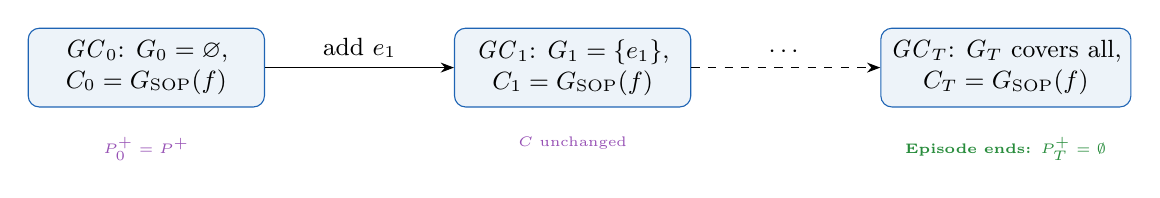
\begin{tikzpicture}[>=Stealth, font=\small,
    every node/.style={align=center}]
  \node[draw=accentblue, rounded corners, minimum width=3cm,
        minimum height=1cm, fill=accentblue!8] (s0)
    {$\GC[0]$: $G_0 = \varnothing$,\\ $C_0 = G_{\mathrm{SOP}}(f)$};

  \node[draw=accentblue, rounded corners, minimum width=3cm,
        minimum height=1cm, fill=accentblue!8, right=2.4cm of s0] (s1)
    {$\GC[1]$: $G_1 = \{e_1\}$,\\ $C_1 = G_{\mathrm{SOP}}(f)$};

  \node[draw=accentblue, rounded corners, minimum width=3cm,
        minimum height=1cm, fill=accentblue!8, right=2.4cm of s1] (sT)
    {$\GC[T]$: $G_T$ covers all,\\ $C_T = G_{\mathrm{SOP}}(f)$};

  \draw[->] (s0) -- node[above]{\small add $e_1$} (s1);
  \draw[->, dashed] (s1) -- node[above]{\small $\cdots$} (sT);

  \node[below=0.25cm of s0, font=\tiny, text=comp_col]
    {$\Pplus_0 = \Pplus$};
  \node[below=0.25cm of s1, font=\tiny, text=comp_col]
    {$C$ unchanged};
  \node[below=0.25cm of sT, font=\tiny, text=int_col]
    {\textbf{Episode ends: $\Pplus_T = \emptyset$}};
\end{tikzpicture}
\end{center}

\subsection{Action Space}

Each action is a triple
\[
  a_t = \bigl(\mathrm{src},\;\mathrm{drn},\;\ell\bigr)
  \;\in\;
  \VG[t] \;\times\; \bigl(\VG[t] \cup \{\nnew\}\bigr)
  \;\times\; \mathcal{L},
\]
where $\nnew$ denotes a fresh internal node to be instantiated.
The action is subject to two structural constraints enforced before
any literal is selected:

\paragraph{Distinctness constraint.}
Transistors are undirected, so $(u,v,\ell)$ and $(v,u,\ell)$ denote the
same device.  At generation time the only structural requirement is that
the two endpoints differ,
\[
  \mathrm{valid\_drn}(\mathrm{src})
  = \bigl(\VG[t] \cup \{\nnew\}\bigr) \setminus \{\mathrm{src}\},
\]
with the source additionally restricted to nodes that are reachable from
$\SOURCE$ or $\SINK$ under at least one still-uncovered on-pattern
(a node that no uncovered pattern can reach cannot contribute coverage).
Duplicate orientations are eliminated not by an index rule but by the
canonical \emph{construction order} used to linearize reference networks
during supervision, defined next.

\paragraph{Construction order (supervision linearization).}
\label{par:order}
Training supervision requires a canonical linearization
$\ell_1,\dots,\ell_R$ of the $R$ undirected transistors of a reference
network into a sequence of MDP actions.  We use a \emph{path (ear)
decomposition}: the sequence is generated by successive walks, where the
first walk starts at $\SOURCE$ and extends through unvisited nodes until
it closes into already-visited structure (preferentially at $\SINK$),
and each subsequent walk (an \emph{ear}) starts at an already-visited
node and again extends until it reconnects.  Formally, each emitted
action $(\mathrm{src},\mathrm{drn},\ell)$ satisfies the invariant that
$\mathrm{src}$ is already present in the partial network, so the walk
direction — not a node-index comparison — fixes the orientation.

This ordering is not merely a tie-breaking convention: it aligns the
supervision with the semantics of the task.  Because conduction is only
achieved when a $\SOURCE\!\to\!\SINK$ path \emph{closes}, decomposing the
target into completed paths means each label continues a coherent
sub-goal.  A further consequence is structural: during a walk extension
the partial network contains exactly one dangling endpoint, and that
endpoint \emph{is} the next source, so the $\mathrm{src}$ decision is
determined by the graph rather than by an arbitrary indexing convention.
The residual difficulty is concentrated at \emph{ear starts}, where the
model must decide from which existing node to branch the next path —
which is precisely the structure-sharing decision that governs network
compactness.  Section~\ref{sec:experiments} quantifies the effect: replacing
an index-based breadth-first linearization with this path decomposition
raises source-selection accuracy from $0.63$ to $0.93$ on $4$-input
functions and from $0.50$ to $0.91$ on $6$-input functions, at identical
model capacity.

\paragraph{Safety mask (BFS cutoff).}
Once $(\mathrm{src}, \mathrm{drn})$ is fixed, any literal whose
addition would create a $\SOURCE \to \SINK$ path under any
$\pi \in \Pminus$ is forbidden:
\[
  \mathcal{F}(\mathrm{src}, \mathrm{drn})
  = \bigl\{\ell \in \mathcal{L} :
      \exists\, \pi \in \Pminus,\;
      \SOURCE \to \SINK
      \text{ in } \bigl(\VG[t],\,\EG[t] \cup \{(\mathrm{src},\mathrm{drn},\ell)\}\bigr)
      \text{ under } \pi
    \bigr\}.
\]
Only literals in $\mathcal{L} \setminus \mathcal{F}(\mathrm{src},\mathrm{drn})$
are allowed.

\subsection{Transition}

Given action $a_t = (\mathrm{src}, \mathrm{drn}, \ell)$:

\begin{enumerate}[leftmargin=1.8em, label=\textbf{\arabic*.}]
  \item \textbf{Update synthesized network.}
    If $\mathrm{drn} = \nnew$, create a new node $n_k$ and
    set $\mathrm{drn} \leftarrow n_k$:
    \[
      \EG[t{+}1] = \EG[t] \cup \{(\mathrm{src},\,\mathrm{drn},\,\ell)\},
      \qquad
      \VG[t{+}1] = \VG[t] \cup \{\mathrm{drn}\}.
    \]

  \item \textbf{Coverage check on $G_{t+1}$ only.}
    Find newly covered on-patterns:
    \[
      \Delta_t
      = \bigl\{\pi \in \Pplus_t :
          \SOURCE \to \SINK
          \text{ in } G_{t+1} \text{ under } \pi
        \bigr\}.
    \]

  \item \textbf{Update coverage tracking.}
    Record newly covered on-patterns:
    \[
      \Pplus_{t+1} = \Pplus_t \setminus \Delta_t.
    \]
    The compensate network is \emph{not} modified:
    $C_{t+1} = G_{\mathrm{SOP}}(f)$.

  \item \textbf{New unified state.}
    $\GC[t{+}1] = G_{t+1} \cup C_{t+1}$.
\end{enumerate}

\begin{notebox}
\textbf{Implementation note.}
The BFS safety check (step 2 of the action selection) must use
$\EG[t]$ only — not the combined $\EG[t] \cup \EC[t]$.  Compensate
transistors represent coverage obligations, not physical switches in
the circuit.  The implementation must therefore maintain $\EG[t]$ and
$\EC[t]$ as separate edge sets, even though $\GC[t]$ presents them
as a single unified graph to the policy.
\end{notebox}

\subsection{Termination}

The episode terminates when $\Pplus_t = \emptyset$, i.e.\ when
$G_t$ routes $\SOURCE \to \SINK$ under every $\pi \in \Pplus$.
The compensate network $C_t = G_{\mathrm{SOP}}(f)$ is present but
no longer contributes new obligations.  At that point:
\begin{itemize}[leftmargin=1.5em, itemsep=2pt]
  \item \textbf{Correctness:} $G_T$ routes $\SOURCE \to \SINK$ under
    every $\pi \in \Pplus$ (since $\Pplus_T = \emptyset$ means all
    patterns were covered during the episode).
  \item \textbf{Safety:} $G_T$ never routes $\SOURCE \to \SINK$
    under any $\pi \in \Pminus$ (guaranteed by the BFS mask at every
    step, by induction from Corollary~\ref{cor:safety}).
\end{itemize}

No explicit ``stop'' action is required.

% ================================================================
\section{Policy Parameterization and Imitation Pretraining}
\label{sec:pretrain}

\subsection{Factorized Policy}

The unified state $\GC[t]$ is encoded by a message-passing network,
producing a node embedding $h_v \in \mathbb{R}^{d}$ for every
$v \in \GC[t]$ and a graph embedding $g \in \mathbb{R}^{2d}$.  The
virtual node $\nnew$ is represented by a learned embedding
$h_{\nnew}$, so that creating a fresh internal node is an ordinary
choice in the same action space.

An action is emitted by four heads applied in sequence, each
conditioned on the previous choices:
\[
  \pi_\theta(a_t \mid \GC[t])
  = \underbrace{\pi^{\mathrm{src}}}_{\text{which node}}
    \cdot
    \underbrace{\pi^{\mathrm{drn}}}_{\text{which partner}}
    \cdot
    \underbrace{\pi^{\mathrm{var}}}_{\text{which variable}}
    \cdot
    \underbrace{\pi^{\mathrm{sgn}}}_{\text{polarity}} .
\]
The source head scores every candidate node, the drain head scores
candidates conditioned on the chosen source, and the variable and
polarity heads select the literal $\ell$ conditioned on both endpoints.
Structural masks (distinctness, reachability) and the safety mask
$\mathcal{F}$ of the action space are applied as
$-\infty$ logit offsets before each softmax, so every sampled action is
admissible by construction and the safety invariant of
Corollary~\ref{cor:safety} holds for all rollouts.

\subsection{Prefix Supervision}

Given a reference network linearized as $\ell_1,\dots,\ell_R$ by the
path decomposition of Section~\ref{par:order}, every prefix
$k = 0,\dots,R-1$ yields one training example: the input is the state
$\GC[k]$ induced by the first $k$ transistors together with the full
compensate network, and the target is the action $\ell_{k+1}$.  A
network with $R$ transistors therefore contributes $R$ supervised
decisions.  Training minimizes the factorized negative log-likelihood
\[
  \mathcal{L}(\theta)
  = -\!\!\sum_{k}\Bigl[
      w_{\mathrm{src}} \log \pi^{\mathrm{src}}_\theta
    + \log \pi^{\mathrm{drn}}_\theta
    + \log \pi^{\mathrm{var}}_\theta
    + \log \pi^{\mathrm{sgn}}_\theta
    \Bigr],
\]
where $w_{\mathrm{src}}$ optionally up-weights the source term, which
empirically dominates the residual loss.

\begin{notebox}
\textbf{Label consistency.}
A Boolean function typically admits many distinct optimal or near-optimal
networks.  If several implementations of the \emph{same} function are all
retained as supervision, identical states are paired with conflicting
targets and the objective acquires an irreducible floor.  Retaining a
single implementation per function (the most compact one) removes this
conflict; Section~\ref{sec:experiments} quantifies the effect.
\end{notebox}

% ================================================================
\section{Network Reduction}
\label{sec:reduction}

A generated network may contain transistors that do not affect the
function it computes.  Two nested notions of reduction are useful; both
are applied before a network's cost is reported.

\begin{definition}[Topological reduction]
A transistor is \emph{structurally dead} if it lies on no simple
$\SOURCE\!\to\!\SINK$ path.  Such transistors cannot participate in any
conduction path and may be deleted.  The reduced network is obtained by
keeping exactly those edges whose biconnected block lies on the
block-cut-tree path between $\SOURCE$ and $\SINK$.
\end{definition}

\begin{definition}[Functional reduction]
A network is \emph{irredundant} if no single transistor can be deleted
while still covering every on-pattern.  A functionally reduced network is
obtained by deleting such transistors greedily until a fixed point.
\end{definition}

\begin{lemma}[Safety is preserved under deletion]
\label{lem:deletion}
Let $G' \subseteq G$ be obtained by deleting transistors.  If $G$ is safe
(routes $\SOURCE\!\to\!\SINK$ under no $\pi \in \Pminus$), then $G'$ is
safe.
\end{lemma}
\begin{proof}
Every path in $G'$ is a path in $G$.  If $G'$ conducted under some
$\pi \in \Pminus$, the same path would conduct in $G$, contradicting
safety of $G$.
\end{proof}

Lemma~\ref{lem:deletion} is what makes functional reduction cheap:
deletion can only \emph{reduce} conduction, so no off-pattern check is
required and it suffices to re-verify on-pattern coverage.  We write
$T_{\mathrm{eff}}(G)$ for the size of the reduced network and use it as
the cost of $G$ throughout, both when reporting results and inside the
reinforcement-learning reward.  Reporting unreduced sizes systematically
overstates cost: on the $6$-input benchmark of
Section~\ref{sec:experiments}, functional reduction lowers the mean
generated size from $41.4$ to $19.0$ transistors.

% ================================================================
\section{Reinforcement Learning Formulation}
\label{sec:rl}

Imitation pretraining optimizes agreement with a particular reference
construction, not the design objective itself.  We therefore finetune the
pretrained policy per target function with policy-gradient updates whose
reward is the quantity we actually care about.

\subsection{Shaped Coverage Reward}

Terminal-only rewards are uninformative when the policy rarely completes
a network: every rollout scores zero and no gradient survives.  We
therefore award partial credit for coverage.  For a rollout producing
network $G$ with $|\Pplus|$ on-patterns in total,
\[
  r(G) =
  \begin{cases}
    w\,\dfrac{|\text{covered}|}{|\Pplus|}, & G \text{ incomplete},\\[1.1em]
    w + (1-w)\,\dfrac{T_{\mathrm{ref}}}{T_{\mathrm{eff}}(G)},
      & G \text{ complete},
  \end{cases}
\]
with $w \in (0,1)$.  Complete networks always out-score incomplete ones,
and among complete networks the reward increases as the network shrinks.

\begin{notebox}
\textbf{Self-tightening reference.}
$T_{\mathrm{ref}}$ is \emph{not} an externally supplied optimum: it is the
smallest reduced size the policy has itself produced for this function so
far.  Matching one's own record scores exactly $1$, beating it scores
above $1$, and regressing scores below.  As the policy improves, the bar
rises automatically, so no oracle cost is needed during training.
\end{notebox}

\subsection{Advantage Estimation}

Let $r_1,\dots,r_K$ be the rewards of $K$ rollouts drawn for the same
target.  The group-relative (critic-free) estimator uses the batch as its
own baseline,
$A_i = (r_i - \bar r)/(\sigma_r + \varepsilon)$.
This is simple but has a structural failure mode: once the policy
converges so that all $K$ rollouts produce the same network,
$\sigma_r \to 0$ and $A_i \to 0$, so learning halts even if the converged
network is suboptimal.  Two remedies are used.

\paragraph{Absolute anchoring.}
Adding a term $\beta\,(r_i - 1)$ re-introduces an absolute scale, so a
group that is uniformly worse than its own record receives uniformly
negative advantage instead of none.

\paragraph{Learned critic with dense credit.}
Alternatively, each placement is rewarded by its own contribution,
$r_t = \alpha\,\Delta\text{coverage}_t - c_{\mathrm{step}}$, with a
completion bonus at the final step, and advantages are formed against a
learned value function, $A_t = R_t - V_\phi(s_t)$.  Because the baseline
is a function of the state rather than of the batch, it does not
degenerate when rollouts agree.  A self-imitation term additionally
replays the best trajectory found so far with positive-part advantage,
consolidating rare discoveries.

\subsection{Escaping Converged Local Optima}
\label{sec:escape}

Even with a non-degenerate baseline, a policy that has converged one
transistor above the optimum receives almost no gradient toward the
optimum, because the reward difference $T_{\mathrm{ref}}/T_{\mathrm{eff}}$
between an $n$- and an $(n{-}1)$-transistor solution is small, while the
self-imitation term actively reinforces the incumbent.  We use three
countermeasures: a \emph{novelty} bonus for producing a structurally
unseen complete network, a discrete bonus for strictly beating the
running record, and down-weighting self-imitation while the record
remains above the target.  A scheduler additionally re-heats the sampling
temperature and entropy coefficient whenever the record stalls, and cools
it again on improvement.

% ================================================================
\section{Experiments}
\label{sec:experiments}

\subsection{Setup}

We evaluate on exhaustive sweeps of $3$- and $4$-input Boolean functions
and on a catalog of $6$-input non-series-parallel (NSP) functions.  Each
function contributes two synthesis targets, the pull-down network
realizing $f$ and the pull-up network realizing $\neg f(\neg x)$.
Reference costs are the minimum-transistor solutions from an exhaustive
SAT-based sweep; a target counts as \emph{solved} when the policy
produces a correct network whose reduced size $T_{\mathrm{eff}}$ meets or
beats that reference.

\subsection{Construction Order Dominates Architecture}

Table~\ref{tab:order} isolates the effect of the supervision
linearization of Section~\ref{par:order}.  Under an index-based
breadth-first order, source-selection accuracy saturates near $0.5$--$0.6$
regardless of model size; under the path decomposition it exceeds $0.88$
with the same encoders.  The ordering contributes roughly $+30$ accuracy
points, while doubling model width contributes $4$--$8$.

\begin{table}[t]
\centering
\caption{Source-selection accuracy on $4$-input functions
(architecture $\times$ supervision order).}
\label{tab:order}
\begin{tabular}{lcc}
\toprule
Architecture & Breadth-first order & Path order \\
\midrule
Base   & $0.543$ & $0.886$ \\
Wide + attention & $0.625$ & $\mathbf{0.932}$ \\
\bottomrule
\end{tabular}
\end{table}

The same effect appears at $6$ inputs, where accuracy rises from $0.505$
to $0.91$.  We attribute this to the structural determinism argued in
Section~\ref{par:order}: under the path order the source is fixed by the
graph during walk extensions, whereas under an index-based order it is an
arbitrary convention the model must memorize.

\subsection{Label Consistency}

Retaining every implementation of a function in the supervision set
introduces conflicting targets for identical states.  On the $6$-input
sweep, restricting supervision to one implementation per function raises
source accuracy from $0.443$ to $0.505$ and, unlike the multi-implementation
setting, the loss continues to decrease rather than degrading.

\subsection{Transistor-Count Optimization}

\paragraph{$3$-input functions.}
All $254$ functions were synthesized for both polarities ($508$ targets).
The pipeline solves \textbf{$508/508$ ($100\%$)} at the SAT-optimal cost.
Notably $496$ targets ($97.6\%$) are already optimal in the pretrained
policy's first sampled evaluation, with only $12$ requiring
reinforcement learning, each converging within $12$ updates.

\paragraph{$4$-input functions.}
Optimization over the full sweep is in progress; on the targets completed
so far the pipeline reaches the SAT-optimal cost on $88\%$.  A frozen
random subset of $256$ solved targets is retained as a fixed evaluation
set for the physical-optimization experiments.

\paragraph{$6$-input NSP functions.}
On the $53$-function NSP catalog, the pretrained policy alone produces a
correct network for $50/53$ functions, but at a mean reduced cost of
$19.0$ transistors against references near $7$: completion is largely
solved by pretraining, whereas compaction is the task left to
reinforcement learning.

\subsection{Diagnostic Analyses}

\paragraph{Top-$k$ behaviour.}
Although top-$1$ source accuracy is $0.50$ on $6$-input states, the
correct node lies within the top $3$ candidates $78\%$ of the time and
within the top $5$ $89\%$ of the time (mean rank $1.6$ of ${\sim}64$).
Because finetuning samples from the policy rather than taking its argmax,
this is the relevant measure of prior quality.

\paragraph{Where source selection fails.}
Accuracy is $0.62$ on small partial networks but falls to $0.36$ on
mid-sized ones, and is markedly lower when the target is an interior node
($0.37$) than a rail ($0.66$); the model over-predicts rails.  Errors are
generally not near-misses, and the model is confidently wrong rather than
undecided, indicating a learning rather than a tie-breaking failure.

\paragraph{Representational ceiling.}
A Weisfeiler--Leman refinement over the state graphs assigns every
candidate node a unique colour within two rounds, so the achievable
source accuracy is $1.0$: the observed gap is an optimization and
inductive-bias limitation, not a representational one.

\paragraph{Cost of the reinforcement-learning variants.}
All reward variants cost essentially the same per update
($\approx 1.6$\,s under identical conditions), since rollout generation
dominates and the critic and exploration mechanisms are negligible in
comparison.  Throughput is instead governed by hardware sharing:
per-update time grows from $1.9$\,s with one process per accelerator to
$20$\,s at five and $49$\,s at sixteen, because each generation step
issues many small kernels that serialize.

% ================================================================
\section{Planned Experiments}
\label{sec:planned}

The following studies are planned to complete the evaluation.

\paragraph{Necessity of pretraining.}
Finetuning from a randomly initialized policy, versus from the pretrained
policy, isolates the contribution of imitation pretraining and validates
the two-stage design.

\paragraph{Component ablation of the escape mechanisms.}
Section~\ref{sec:escape} introduces four mechanisms together; a
leave-one-out study (removing novelty, record-beating bonus,
self-imitation down-weighting, and temperature re-heating in turn) is
required to attribute the gain to individual components.

\paragraph{Variance across seeds.}
Per-target outcomes on hard instances are stochastic: variants have been
observed to exchange wins on the same instance across runs.  All
comparisons will be repeated over multiple seeds and reported with
dispersion rather than as single runs.

\paragraph{Reduction ablation.}
Reporting unreduced, topologically reduced, and functionally reduced
costs side by side quantifies how much of the apparent gap to the
reference is genuine redundancy.

\paragraph{Node features.}
The failure analysis localizes errors to interior nodes of mid-sized
networks.  Supplying per-node structural and functional descriptors
(distance to the rails, degree, and the number of uncovered on-patterns
routed through each node) targets exactly this deficit.

\paragraph{Search budget.}
Completion depends strongly on the step budget; a sweep over budgets
separates failures caused by exhausting the budget from those caused by
an inability to share structure.

\paragraph{Baselines.}
Comparison against the exhaustive SAT reference, a classical
factoring-based synthesizer, and the naive sum-of-products
series-parallel construction places the learned results on a common
scale.

\paragraph{Physical objective.}
The same framework is being extended so that the reward is a
placement-quality metric returned by a layout engine.  Because that
metric is only defined once both the pull-down and pull-up networks are
complete, a target is a \emph{function} rather than a single network, and
the reward is assigned jointly to the two trajectories.

\end{document}
